\documentclass[11pt]{article}
\usepackage[margin=1in]{geometry}
\usepackage[T1]{fontenc}
\usepackage{lmodern}
\usepackage{microtype}
\usepackage{amsmath,amssymb,amsthm}
\usepackage{booktabs}
\usepackage{enumitem}
\usepackage{array}
\usepackage{tikz}
\usetikzlibrary{arrows.meta,positioning,shapes.geometric,fit,calc}
\usepackage{pgfplots}
\pgfplotsset{compat=1.16}
\usepackage[hidelinks]{hyperref}
\usepackage{natbib}
\setcitestyle{authoryear,round}
\setlist{itemsep=2pt,topsep=4pt}

\newtheorem{theorem}{Theorem}
\newtheorem{lemma}{Lemma}
\newtheorem{proposition}{Proposition}
\newtheorem{corollary}{Corollary}
\theoremstyle{definition}
\newtheorem{definition}{Definition}
\newtheorem{axiom}{Axiom}
\theoremstyle{remark}
\newtheorem{remark}{Remark}

\newcommand{\R}{\mathbb{R}}
\newcommand{\Simp}{\Delta}
\newcommand{\one}{\mathbf{1}}
\newcommand{\norm}[1]{\lVert #1\rVert}
\newcommand{\ninf}[1]{\lVert #1\rVert_\infty}
\DeclareMathOperator{\spr}{spread}
\DeclareMathOperator{\softmax}{softmax}

% generated by make_results.py from pytest_output.txt and results.json
\newcommand{\Npassed}{28}
\newcommand{\Nfailed}{0}
\newcommand{\Ntime}{6.28}
\newcommand{\Nprop}{19}
\newcommand{\Ncases}{5700}
\newcommand{\Ncasefail}{0}
\newcommand{\PyVer}{3.13.5}
\newcommand{\PytestVer}{9.1.1}
\newcommand{\HypVer}{6.169.0}
\newcommand{\ExPsi}{-0.238}
\newcommand{\ExDaily}{32.87}
\newcommand{\ExBlend}{34.31}
\newcommand{\EqLiterature}{32.87}
\newcommand{\EqConservative}{34.05}
\newcommand{\EqEqual}{36.00}
\newcommand{\ExRec}{Lumowl (reflection): try Check the Facts}
\newcommand{\DGzero}{0.400}
\newcommand{\DGone}{0.187}
\newcommand{\DGthirty}{2.48\times10^{-4}}
\newcommand{\DGsixty}{3.06\times10^{-7}}
\newcommand{\DGlazythirty}{3.57\times10^{-5}}
\newcommand{\DGsteps}{55}
\newcommand{\LamTwo}{0.8000}
\newcommand{\LamTwoLazy}{0.7500}
\newcommand{\WfourMin}{0.0976}
\newcommand{\DobW}{0.8000}
\newcommand{\DobWfour}{0.4096}
\newcommand{\QBound}{0.5120}
\newcommand{\ConstRes}{4.44\times10^{-16}}
\newcommand{\FJzero}{0.702}
\newcommand{\FJten}{6.04\times10^{-4}}
\newcommand{\FJtwenty}{5.85\times10^{-7}}
\newcommand{\FJforty}{5.57\times10^{-13}}
\newcommand{\RGmeanfour}{1.52\times10^{-1}}
\newcommand{\RGmaxfour}{4.96\times10^{-1}}
\newcommand{\RGboundfour}{0.783}
\newcommand{\RGviolfour}{0}
\newcommand{\RGmedfour}{32}
\newcommand{\RGmaxstepsfour}{110}
\newcommand{\RGmeaneight}{2.78\times10^{-2}}
\newcommand{\RGmaxeight}{2.88\times10^{-1}}
\newcommand{\RGboundeight}{0.732}
\newcommand{\RGvioleight}{0}
\newcommand{\RGmedeight}{36}
\newcommand{\RGmaxstepseight}{144}
\newcommand{\RGmeansixteen}{1.92\times10^{-4}}
\newcommand{\RGmaxsixteen}{6.48\times10^{-3}}
\newcommand{\RGboundsixteen}{0.693}
\newcommand{\RGviolsixteen}{0}
\newcommand{\RGmedsixteen}{28}
\newcommand{\RGmaxstepssixteen}{67}
\newcommand{\UnitRows}{%
Mistfawn & 0.600 & 0.600 & 0.627 & 0.203 & 0.202\\
Tidelyn & 0.400 & 0.400 & 0.478 & 0.174 & 0.179\\
Lumowl & 0.800 & 0.740 & 0.702 & 0.217 & 0.214\\
Brakkor & 0.700 & 0.661 & 0.637 & 0.205 & 0.204\\
Hivewright & 0.700 & 0.662 & 0.619 & 0.201 & 0.201\\
}
\newcommand{\TestRows}{%
\texttt{test\_alpha} & \texttt{test\_softmax\_in\_simplex} & 300 & pass\\
\texttt{test\_alpha} & \texttt{test\_thm2\_blend\_between\_min\_and\_max} & 300 & pass\\
\texttt{test\_alpha} & \texttt{test\_thm3\_lipschitz\_in\_x} & 300 & pass\\
\texttt{test\_alpha} & \texttt{test\_thm4\_lipschitz\_in\_theta} & 300 & pass\\
\texttt{test\_alpha} & \texttt{test\_prop1\_psi\_range\_and\_constants} & -- & pass\\
\texttt{test\_alpha} & \texttt{test\_prop1\_daily\_is\_convex\_blend} & 300 & pass\\
\texttt{test\_alpha} & \texttt{test\_prop1\_daily\_lipschitz} & 300 & pass\\
\texttt{test\_alpha} & \texttt{test\_blended\_daily\_scores\_bounded} & 300 & pass\\
\texttt{test\_mental} & \texttt{test\_creatures\_exact} & -- & pass\\
\texttt{test\_mental} & \texttt{test\_creature\_dag\_counts} & -- & pass\\
\texttt{test\_mental} & \texttt{test\_cycle\_detected} & -- & pass\\
\texttt{test\_mental} & \texttt{test\_thm5\_random\_dag\_terminates\_with\_exact\_counts} & 300 & pass\\
\texttt{test\_mental} & \texttt{test\_thm6\_bounded\_and\_nonexpansive} & 300 & pass\\
\texttt{test\_mental} & \texttt{test\_creature\_needs\_and\_activations\_in\_unit\_interval} & 300 & pass\\
\texttt{test\_peace} & \texttt{test\_thm7\_spread\_monotone\_and\_contracts} & 300 & pass\\
\texttt{test\_peace} & \texttt{test\_thm7\_converges\_to\_pi\_weighted\_consensus} & 300 & pass\\
\texttt{test\_peace} & \texttt{test\_metropolis\_doubly\_stochastic\_gives\_average} & 300 & pass\\
\texttt{test\_peace} & \texttt{test\_creature\_harmony\_matrices} & -- & pass\\
\texttt{test\_peace} & \texttt{test\_thm8\_nash\_unique\_pareto} & 300 & pass\\
\texttt{test\_peace} & \texttt{test\_thm9\_banach\_contraction} & 300 & pass\\
\texttt{test\_pipeline} & \texttt{test\_thm10\_pipeline\_bounded} & 300 & pass\\
\texttt{test\_pipeline} & \texttt{test\_thm10\_settled\_activation\_is\_1\_lipschitz} & 300 & pass\\
\texttt{test\_pipeline} & \texttt{test\_crisis\_gate\_blocks\_scoring} & -- & pass\\
\texttt{test\_veritas} & \texttt{test\_constant\_identities} & -- & pass\\
\texttt{test\_veritas} & \texttt{test\_constants\_are\_immutable} & -- & pass\\
\texttt{test\_veritas} & \texttt{test\_value\_weights\_are\_normalized\_psi\_weights} & -- & pass\\
\texttt{test\_veritas} & \texttt{test\_random\_update\_sequences\_preserve\_invariants} & 300 & pass\\
\texttt{test\_veritas} & \texttt{test\_simplex\_projection\_is\_idempotent\_and\_optimal} & 300 & pass\\
}


\title{\textbf{Project Veda: A Unified Mathematical Framework\\ for a Personal Reflection Operating System}}
\author{Ryan Espinosa}
\date{October 2026}

\begin{document}
\maketitle

\begin{center}
\emph{All credit and glory to God. I owe my knowledge to my Lord Jesus Christ.}
\end{center}
\vspace{4pt}

\begin{abstract}
\noindent Project Veda is a unified mathematical framework that brings four systems together into a personal operating system for reflecting on consciousness, identity, and universal mathematical principles. \textbf{Veritas Aeterna} supplies fixed constants. \textbf{Project Alpha} supplies the mechanism that blends equations. \textbf{Mental Project} supplies a mental architecture whose processing units are pictured as creatures. \textbf{Peaceful Division} supplies harmony layers that settle conflicts between those units. These names and pictures are \emph{philosophical framings}. This paper does not claim to model, measure, or prove anything about consciousness, the soul, or metaphysical truth. What it does is turn each system into ordinary mathematics and prove real properties of that mathematics. Veritas Aeterna becomes a set of axioms, namely real mathematical constants and a normalized value-weight vector on the probability simplex, and we prove that every admissible update preserves the invariants. Project Alpha becomes a softmax-weighted convex blend of component equations, which we prove stays between its components and is Lipschitz in both its inputs and its weights. The MindFrame $\Psi$ index, $\Psi = 0.18C + 0.14S + 0.12M - 0.26R - 0.31B$, turns out to be an exact instance: its Daily Score is a convex blend of oriented terms. Mental Project becomes message passing on a directed acyclic graph of five creature units (Lumowl, Brakkor, Mistfawn, Hivewright, Tidelyn). We prove that a pass terminates with exact cost, stays bounded, and does not amplify differences. Peaceful Division becomes DeGroot averaging, for which we give a self-contained proof of convergence to consensus in the style of Perron--Frobenius; anchored Friedkin--Johnsen averaging, which converges by the Banach fixed-point theorem; and a weighted Nash bargaining rule, which we prove has a unique, Pareto-optimal solution. We then prove that the full pipeline has bounded output and that its iteration converges. A Python package, \texttt{veda}, implements every construction. Its test suite checks each theorem numerically, and in the run reported here all \Npassed{} tests passed, including \Nprop{} randomized property tests that covered \Ncases{} generated cases with \Ncasefail{} failures. Veda is a self-reflection aid. It is not therapy and it is not a diagnosis. In a crisis in the US, call or text 988.
\end{abstract}

\tableofcontents
\newpage

%=====================================================================
\section{Introduction}
Many people keep a private ``inner operating system'': habits of attention, values they try to keep fixed, ways of weighing competing urges, and ways of making peace inside themselves. Project Veda tries to write such a system down precisely enough that a computer can run it and a reader can check it. It joins four earlier ideas from the author:

\begin{enumerate}
\item \textbf{Veritas Aeterna} (``eternal truth''): some things should not drift, namely a person's normalized value weights and the constants of mathematics.
\item \textbf{Project Alpha}: many component equations, blended into one.
\item \textbf{Mental Project}: the mind pictured as a society of small processing units, here drawn as five invented creatures.
\item \textbf{Peaceful Division}: when units disagree, the disagreement is settled by a fair and provably convergent process, not by one unit overpowering the rest.
\end{enumerate}

\paragraph{Epistemic status (please read).} The four names, the creatures, and the phrase ``consciousness framework'' are \textbf{philosophical and mnemonic framings}. The paper does not claim that these mathematical objects \emph{are} consciousness, that they explain subjective experience \citep[the ``hard problem'';][]{chalmers1995}, or that they establish any metaphysical or theological truth. The theorems are about the equations themselves: bounds, invariants, termination, and convergence. They tell us that the software behaves predictably. They tell us nothing about whether it helps anyone. The psychological inputs come from the MindFrame $\Psi$ index \citep{espinosa2026mindframe}, which is an unvalidated heuristic. The author's faith is stated in the dedication as a personal confession. It is not offered as a result of the mathematics, and the mathematics does not depend on it.

\paragraph{Contributions.}
(i)~A formalization of each of the four systems (Sections~\ref{sec:veritas}--\ref{sec:peace}).
(ii)~Ten theorems and one proposition, each with a complete proof (Table~\ref{tab:theorems}).
(iii)~An integrated pipeline whose output is provably bounded and whose iteration provably converges (Section~\ref{sec:integration}).
(iv)~A working Python prototype with a test suite that checks each proven property, and the actual results of running it (Section~\ref{sec:prototype}).
(v)~Limitations, a safety note, and a path to MindFrame $\Psi$-Lab (Sections~\ref{sec:limits}--\ref{sec:future}).

\begin{figure}[t]
\centering
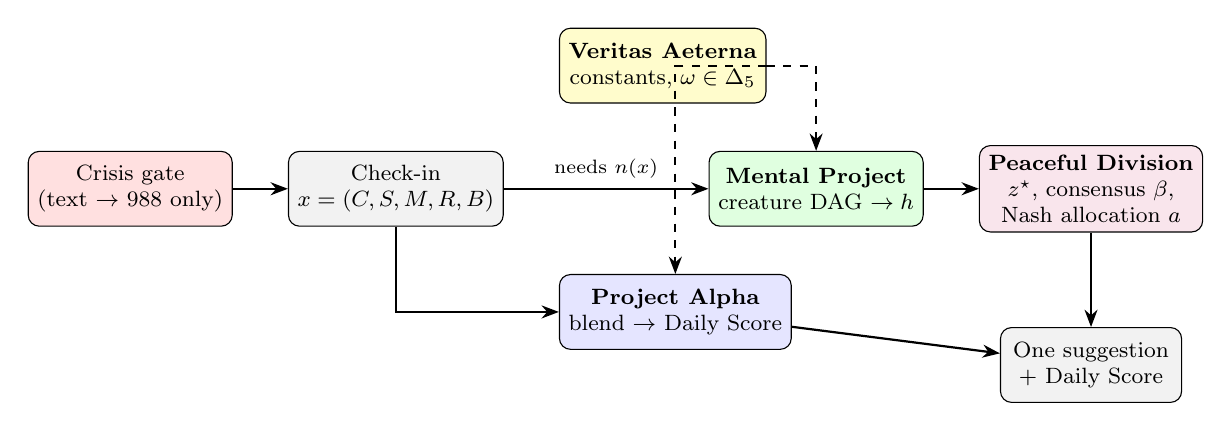
\begin{tikzpicture}[
  box/.style={draw,rounded corners,align=center,minimum width=2.3cm,minimum height=0.95cm,font=\footnotesize},
  arr/.style={-{Stealth[length=2.2mm]},thick}]
\node[box,fill=red!12] (gate) {Crisis gate\\(text $\to$ 988 only)};
\node[box,fill=gray!10,right=7mm of gate] (x) {Check-in\\$x=(C,S,M,R,B)$};
\node[box,fill=yellow!20,above right=6mm and 7mm of x] (va) {\textbf{Veritas Aeterna}\\constants, $\omega\in\Simp_5$};
\node[box,fill=blue!10,below right=6mm and 7mm of x] (pa) {\textbf{Project Alpha}\\blend $\to$ Daily Score};
\node[box,fill=green!12,right=26mm of x] (mp) {\textbf{Mental Project}\\creature DAG $\to h$};
\node[box,fill=purple!10,right=7mm of mp] (pd) {\textbf{Peaceful Division}\\$z^\star$, consensus $\beta$,\\Nash allocation $a$};
\node[box,fill=gray!10,below=12mm of pd] (out) {One suggestion\\+ Daily Score};
\draw[arr] (gate) -- (x);
\draw[arr] (x) -- node[above,font=\scriptsize]{needs $n(x)$} (mp);
\draw[arr] (x) |- (pa);
\draw[arr,dashed] (va) -| (mp);
\draw[arr,dashed] (va) -| (pa.north);
\draw[arr] (mp) -- (pd);
\draw[arr] (pd) -- (out);
\draw[arr] (pa) -- (out);
\end{tikzpicture}
\caption{Veda architecture. Dashed arrows show where the fixed constants of Veritas Aeterna are used; Theorem~\ref{thm:veritas} guarantees that no stage changes them or pushes the state outside its invariant set. Crisis text bypasses everything.}
\label{fig:arch}
\end{figure}

\paragraph{Notation.} $\Simp_n=\{w\in\R^n: w_i\ge 0,\ \sum_i w_i=1\}$ is the probability simplex, and $\operatorname{int}\Simp_n$ is the subset with all $w_i>0$. We write $\ninf{v}=\max_i|v_i|$ and $\spr(v)=\max_i v_i-\min_i v_i$. For a matrix $P$ with columns of opinions, $\spr(P)$ is the largest spread over columns. A matrix is \emph{row-stochastic} if it has nonnegative entries and every row sums to~1. $\one$ is the all-ones vector.

\begin{table}[t]
\centering\small
\begin{tabular}{@{}l l p{9.6cm}@{}}
\toprule
\# & System & Statement (informal)\\
\midrule
Thm~\ref{thm:veritas} & Veritas & Every finite sequence of admissible updates keeps $(w,x)\in\Simp_n\times[0,1]^m$.\\
Thm~\ref{thm:bounds} & Alpha & A softmax blend lies between its smallest and largest component, strictly unless they are all equal.\\
Thm~\ref{thm:lipx} & Alpha & The blend is $(\sum_i\alpha_iL_i)$-Lipschitz in $x$, so at most $\max_i L_i$.\\
Thm~\ref{thm:liptheta} & Alpha & $|B_\theta-B_{\theta'}|\le \frac{s}{2\tau}\ninf{\theta-\theta'}$, where $s$ is the spread of the components.\\
Prop~\ref{prop:psi} & Alpha & Daily Score $=100\,\omega^\top y$ with $\omega=|w|/1.01\in\Simp_5$, so it lies in $[0,100]$ and is $100$-Lipschitz in $\ninf{\cdot}$.\\
Thm~\ref{thm:term} & Mental & Kahn's pass halts. It succeeds if and only if the graph is acyclic, and then costs exactly $|V|$ evaluations and $|E|$ messages.\\
Thm~\ref{thm:mentalbound} & Mental & Unit outputs lie in $[\min n,\max n]\subseteq[0,1]$, and $n\mapsto h$ is non-expansive.\\
Lemma~\ref{lem:primitive}, Thm~\ref{thm:degroot} & Peace & DeGroot averaging converges geometrically to the consensus $\pi^\top p(0)$, with $\pi>0$ unique.\\
Thm~\ref{thm:nash} & Peace & The weighted Nash bargaining solution is unique, Pareto-optimal, and has the closed form $d+\beta(1-\sum d)$.\\
Thm~\ref{thm:fj} & Peace & Anchored averaging is a $\mu$-contraction with a unique, bounded, 1-Lipschitz fixed point.\\
Thm~\ref{thm:integration} & All & The integrated pipeline is bounded and well defined, its iteration converges, and $x\mapsto z^\star$ is 1-Lipschitz.\\
\bottomrule
\end{tabular}
\caption{Results proved in this paper. Each one is checked numerically by named tests (Table~\ref{tab:tests}).}
\label{tab:theorems}
\end{table}

%=====================================================================
\section{Related Work and Caveats}\label{sec:related}
\textbf{Society of Mind.} \citet{minsky1986} proposed that minds are made of many simple ``agents'' whose interactions produce intelligence. Mental Project borrows this picture. Minsky's book is a speculative theory, not an empirically validated model, and our five creatures are a design device, not a claim about brain anatomy.

\textbf{Global workspace theory.} \citet{baars1988} proposed that conscious contents are those broadcast from a limited-capacity ``workspace'' to many specialized processors. Our consensus step looks a little like a broadcast, but Veda has no workspace dynamics, no competition for access, and no claim to model conscious access. Global workspace theory itself remains one of several contested scientific theories of consciousness.

\textbf{Integrated information theory.} \citet{tononi2004} and \citet{tononi2016} propose that consciousness corresponds to integrated information, $\Phi$. Veda computes nothing resembling $\Phi$, and we make no claim that its ``integration'' (function composition) has anything to do with IIT's. IIT is also highly controversial: in 2023 a large group of researchers publicly criticized it as unfalsifiable \citep{fleming2023}, and others have disputed that criticism.

\textbf{Consensus and social influence.} \citet{degroot1974} modeled a group reaching consensus by repeated weighted averaging of opinions. \citet{friedkin1990} added ``stubbornness,'' an anchoring to initial opinions, which in general prevents full consensus. Convergence of products of stochastic matrices is classical \citep{seneta2006}, and the coefficient of ergodicity we use goes back to \citet{dobrushin1956}. Metropolis--Hastings weights for distributed averaging are analyzed in \citet{xiao2004}.

\textbf{Perron--Frobenius and Banach.} The Perron--Frobenius theorem \citep{perron1907,frobenius1912} guarantees a positive leading eigenvector for nonnegative irreducible matrices. We prove the part we need directly, with a contraction argument (Theorem~\ref{thm:degroot}). The Banach fixed-point theorem \citep{banach1922} gives Theorem~\ref{thm:fj}.

\textbf{Bargaining.} \citet{nash1950} characterized the bargaining solution that maximizes the product of utility gains. \citet{kalai1977} studied the asymmetric (weighted) version that we use.

\textbf{Blending and projection.} Softmax-weighted mixtures are standard. \citet{gao2017} study Lipschitz properties of the softmax map itself, and we prove a sensitivity bound for the blended \emph{output}. Euclidean projection onto the simplex follows \citet{held1974} and \citet{duchi2008}. The multiplicative update is the exponentiated-gradient step of \citet{kivinen1997}.

\textbf{MindFrame and DBT.} The five input terms and the $\Psi$ index come from the author's MindFrame paper \citep{espinosa2026mindframe}. The skills each creature suggests (Check the Facts, Opposite Action, TIPP) are named in the DBT skills manual \citep{linehan2015}, while ``one easy skill'' and ``reach out'' are plain-language prompts. A suggestion from Veda is not DBT, which is taught inside a structured clinical program.

\textbf{Testing.} Property-based testing goes back to QuickCheck \citep{claessen2000}. We use the Python library Hypothesis \citep{maciver2019}.

%=====================================================================
\section{Veritas Aeterna: Fixed Constants and Invariants}\label{sec:veritas}
\begin{axiom}[Mathematical constants]\label{ax:const}
The constants $\pi$, $e$, $\varphi=(1+\sqrt5)/2$ and $\sqrt2$ are fixed. They satisfy $\varphi^2=\varphi+1$, $e^{i\pi}+1=0$, $\ln e=1$ and $(\sqrt2)^2=2$.
\end{axiom}
These identities are standard mathematics, not results of this paper. In floating point the prototype's largest residual is $\ConstRes$, which is rounding error.

\begin{axiom}[Normalized value weights]\label{ax:omega}
Let $w=(0.18,0.14,0.12,-0.26,-0.31)$ be the MindFrame $\Psi$ weights for $(C,S,M,R,B)$. The \emph{value-weight vector} is $\omega=|w|/\sum_i|w_i|=(18,14,12,26,31)/101\in\operatorname{int}\Simp_5$.
\end{axiom}

\begin{definition}[Invariant set and admissible updates]
The state is $(w,x)$ with $w\in\R^n$ (weights) and $x\in\R^m$ (terms). The invariant set is $\mathcal I=\Simp_n\times[0,1]^m$. The admissible updates are
\textbf{U1} (box) $x\leftarrow \Pi_{[0,1]^m}(v)=\min(\max(v,0),1)$ applied coordinatewise;
\textbf{U2} (simplex) $w\leftarrow\Pi_{\Simp_n}(v)=\arg\min_{u\in\Simp_n}\norm{u-v}_2$;
\textbf{U3} (mix) $(w,x)\leftarrow((1-\lambda)w+\lambda w',\ (1-\lambda)x+\lambda x')$ with $\lambda\in[0,1]$ and $(w',x')\in\mathcal I$;
\textbf{U4} (multiplicative) $w_i\leftarrow w_i e^{\eta g_i}/\sum_j w_je^{\eta g_j}$ with $\eta\ge0$ and $g\in\R^n$.
\end{definition}

\begin{theorem}[Invariant preservation]\label{thm:veritas}
Each of U1--U4 maps $\mathcal I$ into $\mathcal I$. Consequently every finite composition of admissible updates does too. U4 also preserves the support $\{i:w_i>0\}$, and U1--U4 never change the constants of Axioms~\ref{ax:const}--\ref{ax:omega}.
\end{theorem}
\begin{proof}
U1: each coordinate $\min(\max(v_i,0),1)$ lies in $[0,1]$, and $w$ is unchanged.
U2: $\Simp_n$ is nonempty, closed and convex, so by the projection theorem in Hilbert space the minimizer exists, is unique, and belongs to $\Simp_n$; $x$ is unchanged.
U3: $\Simp_n$ and $[0,1]^m$ are convex, so convex combinations of their points stay in them.
U4: if $w\in\Simp_n$, the numerators $w_ie^{\eta g_i}$ are nonnegative and not all zero, because some $w_i>0$ and $e^{\eta g_i}>0$. Dividing by their sum gives a point of $\Simp_n$. A numerator is zero exactly when $w_i=0$, so the support is preserved.
For compositions, induct on the length $k$. The empty composition is the identity. If the state is in $\mathcal I$ after $k$ steps, the $(k+1)$-st update keeps it in $\mathcal I$ by the cases above. None of the updates takes the constants as an argument it can write to. The prototype also stores them in read-only mappings, so an attempt to assign to them raises an error.
\end{proof}

\begin{remark}
``Eternal'' is a framing. Mathematically, Theorem~\ref{thm:veritas} says only that the admissible update set is closed with respect to the invariant set. Immutability of the stored constants is a software property, and the tests check it (Section~\ref{sec:prototype}).
\end{remark}

%=====================================================================
\section{Project Alpha: Blending Component Equations}\label{sec:alpha}
\begin{definition}[Blend]
Let $f_1,\dots,f_k:X\to\R$ be component equations, $\theta\in\R^k$ logits, and $\tau>0$ a temperature. Set $\alpha(\theta)=\softmax(\theta/\tau)$, that is, $\alpha_i=e^{\theta_i/\tau}/\sum_je^{\theta_j/\tau}$, and define $B_\theta(x)=\sum_i\alpha_i(\theta)f_i(x)$.
\end{definition}
Since every $e^{\theta_i/\tau}>0$, we have $\alpha(\theta)\in\operatorname{int}\Simp_k$.

\begin{theorem}[Bounded blend]\label{thm:bounds}
For every $x$, $\min_if_i(x)\le B_\theta(x)\le\max_if_i(x)$. Both inequalities are strict unless all the $f_i(x)$ are equal.
\end{theorem}
\begin{proof}
Let $m=\min_if_i(x)$ and $M=\max_if_i(x)$. Then $B_\theta(x)-m=\sum_i\alpha_i(f_i(x)-m)\ge0$ because $\alpha_i>0$ and $\sum\alpha_i=1$. The sum is $0$ only if every $f_i(x)=m$. The upper bound follows in the same way.
\end{proof}

\begin{theorem}[Lipschitz in the input]\label{thm:lipx}
If $|f_i(x)-f_i(x')|\le L_i\norm{x-x'}$ for some norm, then $|B_\theta(x)-B_\theta(x')|\le\big(\sum_i\alpha_iL_i\big)\norm{x-x'}\le(\max_iL_i)\norm{x-x'}$.
\end{theorem}
\begin{proof}
By the triangle inequality, $|\sum_i\alpha_i(f_i(x)-f_i(x'))|\le\sum_i\alpha_iL_i\norm{x-x'}$. Since $\alpha\in\Simp_k$, $\sum\alpha_iL_i\le\max L_i$.
\end{proof}

\begin{theorem}[Sensitivity to the blending weights]\label{thm:liptheta}
Fix $x$, let $v_i=f_i(x)$, and let $s=\max_iv_i-\min_iv_i$. For all $\theta,\theta'\in\R^k$,
\[|B_\theta(x)-B_{\theta'}(x)|\le\frac{s}{2\tau}\ninf{\theta-\theta'}.\]
\end{theorem}
\begin{proof}
Let $g(\theta)=\alpha(\theta)^\top v$. Differentiating the softmax gives $\partial\alpha_i/\partial\theta_j=\tau^{-1}\alpha_i(\delta_{ij}-\alpha_j)$, so $\partial g/\partial\theta_j=\tau^{-1}\alpha_j(v_j-\bar v)$, where $\bar v=\alpha^\top v$. Hence $\norm{\nabla g}_1=\tau^{-1}\sum_j\alpha_j|v_j-\bar v|$. Let $V$ be a random variable equal to $v_j$ with probability $\alpha_j$, so that $\mathbb E V=\bar v$. By Jensen's inequality, $\mathbb E|V-\bar v|\le\sqrt{\operatorname{Var}V}$. With $c=(\min v+\max v)/2$, the variance is at most $\mathbb E(V-c)^2\le(s/2)^2$, because the mean minimizes expected squared deviation and $|V-c|\le s/2$. So $\norm{\nabla g(\xi)}_1\le s/(2\tau)$ for every $\xi$. By the mean value theorem on the segment from $\theta'$ to $\theta$, $|g(\theta)-g(\theta')|=|\nabla g(\xi)^\top(\theta-\theta')|\le\norm{\nabla g(\xi)}_1\ninf{\theta-\theta'}$.
\end{proof}
In words: raising the temperature, or blending equations that already agree, makes the output less sensitive to how the weights are set.

\subsection{The MindFrame $\Psi$ index as an instance}
\begin{proposition}[$\Psi$ Daily Score is a convex blend]\label{prop:psi}
Let $(C,S,M,R,B)\in[0,1]^5$ and $\Psi=0.18C+0.14S+0.12M-0.26R-0.31B$. Let $y=(C,S,M,1-R,1-B)$ and let $\omega$ be as in Axiom~\ref{ax:omega}. Then
\[\text{Daily Score}=\frac{100(\Psi+0.57)}{1.01}=100\,\omega^\top y .\]
Consequently: (a) $\Psi\in[-0.57,0.44]$ and the Daily Score lies in $[100\min_iy_i,\ 100\max_iy_i]\subseteq[0,100]$. (b) The score is $0$ only at $(0,0,0,1,1)$ and $100$ only at $(1,1,1,0,0)$. (c) $|\Delta\text{Daily}|\le\frac{100}{1.01}\sum_i|w_i||\Delta x_i|\le100\ninf{\Delta x}$.
(d) The score equals the Project Alpha blend $B_\theta$ with $f_i=100y_i$, $\tau=1$ and $\theta_i=\ln\omega_i$.
\end{proposition}
\begin{proof}
Write $-0.26R=0.26(1-R)-0.26$ and $-0.31B=0.31(1-B)-0.31$. Then $\Psi+0.57=0.18C+0.14S+0.12M+0.26(1-R)+0.31(1-B)=\sum_i|w_i|y_i$, and $\sum|w_i|=1.01$. Dividing by $1.01$ gives the identity. (a) follows from Theorem~\ref{thm:bounds}, using $y\in[0,1]^5$ and $\Psi=1.01\,\omega^\top y-0.57$. For (b), $\omega>0$, so $\omega^\top y=0$ forces $y=0$ and $\omega^\top y=1$ forces $y=\one$. (c) follows from Theorem~\ref{thm:lipx} with $|\Delta y_i|=|\Delta x_i|$ and $\sum_i\omega_i=1$. (d) holds because $\softmax(\ln\omega)=\omega$.
\end{proof}
This gives the earlier, ad hoc rescaling in the MindFrame paper a principled reading: the Daily Score is a weighted average of five ``higher is better'' terms. Prop.~\ref{prop:psi}(c) also gives a useful fact: changing one item by $0.1$ moves the score by at most $100\cdot0.31\cdot0.1/1.01\approx3.07$ points.

\paragraph{Blending three scoring equations.} The prototype also blends the literature-weight Daily Score, the conservative-weight Daily Score from the MindFrame paper \citep{espinosa2026mindframe}, and an equal-weight score $100\,\overline{y}$. For the illustrative example input $x=(0.4,0.6,0.3,0.7,0.8)$, which is \emph{made up} and is not anyone's data, the three equations give $\EqLiterature$, $\EqConservative$ and $\EqEqual$. With $\theta=0$ (equal weights) the blend is $\ExBlend$, which lies between them, as Theorem~\ref{thm:bounds} requires.

%=====================================================================
\section{Mental Project: Creature Units on a DAG}\label{sec:mental}
The five units are invented characters. Each one reads one MindFrame term as a \emph{need} in $[0,1]$ and stands for one suggested skill (Table~\ref{tab:creatures}).

\begin{table}[h]
\centering\small
\begin{tabular}{@{}l p{5.4cm} l c c l@{}}
\toprule
Unit & Image & Virtue & Term & Need $n_u$ & Suggested skill\\
\midrule
Lumowl & a lantern-eyed night watcher & reflection & $B$ & $B$ & Check the Facts\\
Brakkor & a stone-maned beast that walks toward the storm & courage & $R$ & $R$ & Opposite Action\\
Mistfawn & a fog spirit that slows every breath & calm & $C$ & $1-C$ & TIPP\\
Hivewright & a many-armed builder laying one brick a day & discipline & $M$ & $1-M$ & one easy skill\\
Tidelyn & a sea serpent linking far shores & connection & $S$ & $1-S$ & reach out\\
\bottomrule
\end{tabular}
\caption{The five creature units. ``Need'' is high when the term has the most room to improve. Since $n=\one-y$, the map $x\mapsto n$ is 1-Lipschitz in $\ninf{\cdot}$.}
\label{tab:creatures}
\end{table}

\begin{definition}[Creature network]\label{def:dag}
A creature network is a finite directed acyclic graph $G=(V,E)$ with coefficients $a_u>0$ and $b_{uv}\ge0$ for each edge $v\to u$, satisfying $a_u+\sum_{v\in\mathrm{pred}(u)}b_{uv}=1$. Given needs $n\in[0,1]^V$, the unit outputs are
\[h_u=a_un_u+\sum_{v\in\mathrm{pred}(u)}b_{uv}h_v .\]
\end{definition}

The default network (Fig.~\ref{fig:dag}) encodes a \emph{design choice}, not an empirical finding: calm comes first and feeds reflection and courage, connection supports courage and discipline, and courage feeds discipline. The order loosely follows the DBT idea of reducing high arousal (TIPP) before using more demanding skills \citep{linehan2015}.

\begin{figure}[h]
\centering
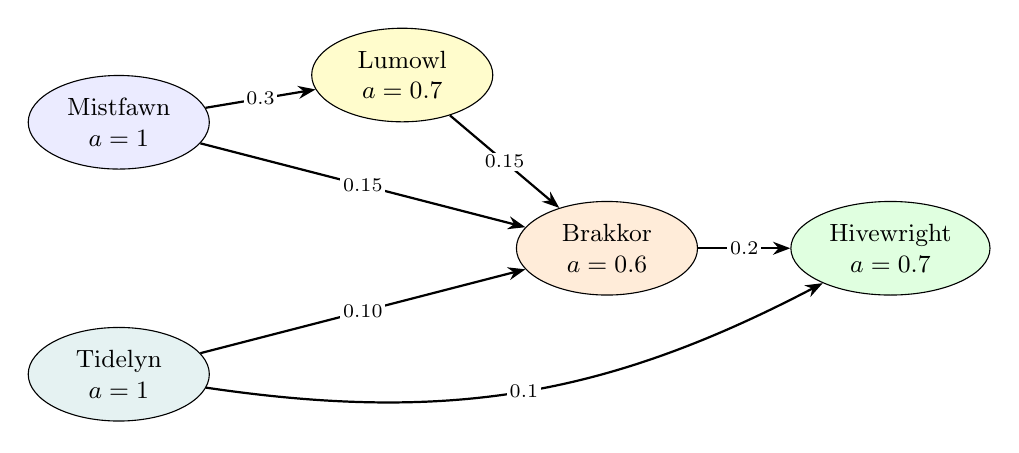
\begin{tikzpicture}[
  u/.style={draw,ellipse,minimum width=2.3cm,minimum height=0.9cm,align=center,font=\small},
  arr/.style={-{Stealth[length=2.2mm]},thick},
  lab/.style={font=\scriptsize,fill=white,inner sep=1pt}]
\node[u,fill=blue!8] (mf) at (0,1.6) {Mistfawn\\$a=1$};
\node[u,fill=teal!10] (td) at (0,-1.6) {Tidelyn\\$a=1$};
\node[u,fill=yellow!20] (lo) at (3.6,2.2) {Lumowl\\$a=0.7$};
\node[u,fill=orange!15] (bk) at (6.2,0) {Brakkor\\$a=0.6$};
\node[u,fill=green!12] (hw) at (9.8,0) {Hivewright\\$a=0.7$};
\draw[arr] (mf) -- node[lab]{0.3} (lo);
\draw[arr] (mf) -- node[lab]{0.15} (bk);
\draw[arr] (lo) -- node[lab]{0.15} (bk);
\draw[arr] (td) -- node[lab]{0.10} (bk);
\draw[arr] (bk) -- node[lab]{0.2} (hw);
\draw[arr] (td) to[bend right=18] node[lab]{0.1} (hw);
\end{tikzpicture}
\caption{The default creature DAG ($|V|=5$, $|E|=6$). Edge labels are $b_{uv}$. Each unit's coefficients sum to 1.}
\label{fig:dag}
\end{figure}

\paragraph{Pass algorithm.} We use Kahn's topological sort \citep{kahn1962}. Start a queue with the units that have in-degree $0$. Repeatedly dequeue a unit $v$, compute $h_v$, and decrement the in-degree of each successor, enqueueing any whose in-degree reaches $0$. If fewer than $|V|$ units are dequeued, report a cycle.

\begin{theorem}[Termination and exact cost]\label{thm:term}
On any finite directed graph the pass halts after at most $|V|$ dequeues. Every unit is dequeued if and only if $G$ is acyclic. In that case each $h_u$ is computed after all $h_v$ with $v\in\mathrm{pred}(u)$, and the pass performs exactly $|V|$ unit evaluations and $|E|$ messages.
\end{theorem}
\begin{proof}
In-degrees only decrease, so each unit's in-degree reaches $0$ at most once and each unit is enqueued at most once. There are therefore at most $|V|$ dequeues, and each one does finitely much work, so the pass halts. Suppose $G$ is acyclic but the set $U$ of units never dequeued is nonempty. Each $u\in U$ ends with positive in-degree. Predecessors outside $U$ were dequeued and already decremented it, so $u$ has a predecessor in $U$. Following predecessors inside the finite set $U$ must eventually repeat a unit, which gives a cycle, a contradiction. Conversely, if $G$ has a cycle, the first unit on the cycle to be dequeued would need in-degree $0$ while its predecessor on the cycle had not yet been dequeued, which is impossible. So no cycle unit is ever dequeued. A unit is dequeued only once its in-degree is $0$, which means all its predecessors were already dequeued and evaluated. Each unit is evaluated once, which gives $|V|$ evaluations, and each edge $v\to u$ contributes exactly one term $b_{uv}h_v$, which gives $|E|$ messages.
\end{proof}

\begin{theorem}[Bounded and non-expansive]\label{thm:mentalbound}
For needs $n\in[0,1]^V$, every output satisfies $\min_vn_v\le h_u\le\max_vn_v$, so $h\in[0,1]^V$. For two need vectors $n,n'$, $\ninf{h(n)-h(n')}\le\ninf{n-n'}$. Also $h_u\ge a_un_u$, so a unit with a large need cannot be pushed below a fixed fraction of it.
\end{theorem}
\begin{proof}
Use strong induction along the topological order of Theorem~\ref{thm:term}. Suppose all predecessors $v$ of $u$ satisfy $h_v\in[m,M]$, where $m=\min n$ and $M=\max n$. Then $h_u$ is a convex combination (weights $a_u,b_{uv}$, summing to 1) of $n_u$ and the $h_v$, all of which lie in $[m,M]$, so $h_u\in[m,M]$. Similarly, if $|h_v-h'_v|\le\delta:=\ninf{n-n'}$ for all predecessors, then $|h_u-h'_u|\le a_u|n_u-n'_u|+\sum b_{uv}|h_v-h'_v|\le(a_u+\sum b_{uv})\delta=\delta$. Finally, $h_u\ge a_un_u$ because every other term is nonnegative.
\end{proof}

%=====================================================================
\section{Peaceful Division: Harmony Layers}\label{sec:peace}
Units disagree. Lumowl wants the next minute spent checking facts, while Brakkor wants it spent approaching what is being avoided. Peaceful Division resolves such disagreements in three layers: \emph{anchored harmony}, in which units listen to neighbors without giving up their own evidence (Friedkin--Johnsen); \emph{consensus}, in which proposals are averaged until they agree (DeGroot); and \emph{fair division}, in which a fixed attention budget is shared by Nash bargaining.

\paragraph{The harmony graph.} Units talk along the edges of Fig.~\ref{fig:dag}, now taken as undirected. Brakkor has degree 4 and the other units have degree 2. We use Metropolis--Hastings weights \citep{xiao2004}, $W_{ij}=1/(1+\max(d_i,d_j))$ on edges and $W_{ii}=1-\sum_{j\ne i}W_{ij}$:
\[
W=\begin{pmatrix}
0.4667&0&0.3333&0.2&0\\
0&0.4667&0&0.2&0.3333\\
0.3333&0&0.4667&0.2&0\\
0.2&0.2&0.2&0.2&0.2\\
0&0.3333&0&0.2&0.4667
\end{pmatrix}
\]
with rows and columns in the order Mistfawn, Tidelyn, Lumowl, Brakkor, Hivewright (entries rounded to four decimals).
$W$ is symmetric, row-stochastic, and has a positive diagonal.

\subsection{DeGroot consensus}
Let $W\in\R^{n\times n}$ be row-stochastic with $W_{ii}>0$ for all $i$, and suppose its graph ($i\to j$ when $W_{ij}>0$) is strongly connected. Opinions evolve by $p(t+1)=Wp(t)$, where $p(t)\in\R^n$, or $\R^{n\times k}$ with the update applied to each column.

\begin{lemma}[Primitivity]\label{lem:primitive}
All entries of $W^{n-1}$ are positive.
\end{lemma}
\begin{proof}
$(W^k)_{ij}$ is a sum over walks of length $k$ from $i$ to $j$ of products of edge weights, so it is positive if at least one such walk exists. For $i\ne j$, strong connectivity gives a shortest path of some length $\ell\le n-1$. Prepending $n-1-\ell$ self-loops at $i$, each with weight $W_{ii}>0$, gives a walk of length exactly $n-1$. For $i=j$, use $n-1$ self-loops.
\end{proof}

\begin{lemma}[Spread contraction]\label{lem:spread}
For row-stochastic $A$, let $\gamma(A)=\min_{i,j}\sum_k\min(A_{ik},A_{jk})$. Then $\spr(Ap)\le(1-\gamma(A))\spr(p)$. If all entries of $A$ are at least $\delta$, then $\gamma(A)\ge n\delta$. Also, $\max(Ap)\le\max p$ and $\min(Ap)\ge\min p$.
\end{lemma}
\begin{proof}
Fix rows $i,j$ and let $c_k=\min(A_{ik},A_{jk})$, with $\gamma_{ij}=\sum_kc_k$. Then $(Ap)_i-(Ap)_j=\sum_k(A_{ik}-c_k)p_k-\sum_k(A_{jk}-c_k)p_k$. Both coefficient vectors are nonnegative and each sums to $1-\gamma_{ij}$, so the difference is at most $(1-\gamma_{ij})\max p-(1-\gamma_{ij})\min p$. Taking the worst pair gives the bound. If all $A_{ik}\ge\delta$, then every $c_k\ge\delta$. Each $(Ap)_i$ is a convex combination of the entries of $p$. (The quantity $1-\gamma$ is Dobrushin's ergodicity coefficient \citep{dobrushin1956,seneta2006}.)
\end{proof}

\begin{theorem}[Consensus]\label{thm:degroot}
Let $\delta=\min_{ij}(W^{n-1})_{ij}>0$ and $q=1-n\delta\in[0,1)$. Then:
(a) $\spr(p(t))$ is non-increasing and $\spr(p(t))\le q^{\lfloor t/(n-1)\rfloor}\spr(p(0))$;
(b) there is a unique $\pi\in\Simp_n$ with $\pi^\top W=\pi^\top$, and it satisfies $\pi_k\ge\delta>0$;
(c) $W^t\to\one\pi^\top$ and $p(t)\to\one\,\pi^\top p(0)$, a consensus that lies in $[\min p(0),\max p(0)]$ in each coordinate.
\end{theorem}
\begin{proof}
$q<1$ by Lemma~\ref{lem:primitive}, and $q\ge0$ because the $n$ entries in a row of $W^{n-1}$ sum to 1. (a) follows from Lemma~\ref{lem:spread}: apply it with $A=W$ at every step (monotonicity), and with $A=W^{n-1}$ every $n-1$ steps (contraction). (c) and (b): $\max p(t)$ is non-increasing and $\min p(t)$ is non-decreasing, both are bounded, and their gap tends to $0$ by (a). So they converge to a common limit $c(p(0))\in[\min p(0),\max p(0)]$, and every coordinate converges to it. The map $p(0)\mapsto c(p(0))$ is a limit of linear maps, so it is linear: $c(p)=\pi^\top p$ with $\pi_k=c(e_k)\in[0,1]$. Since $c(\one)=1$, $\pi\in\Simp_n$. Applying this to $p(0)=e_k$ gives $W^te_k\to\pi_k\one$, that is, $W^t\to\one\pi^\top$. Because the sequence $(W^tWp)_t$ is a shift of $(W^tp)_t$, $c(Wp)=c(p)$, so $\pi^\top W=\pi^\top$. For $t\ge n-1$, $W^t=W^{t-n+1}W^{n-1}$ is a row-stochastic matrix times a matrix with entries $\ge\delta$, so its entries are $\ge\delta$, and hence $\pi_k\ge\delta$. For uniqueness, if $\sigma\in\Simp_n$ and $\sigma^\top W=\sigma^\top$, then $\sigma^\top=\sigma^\top W^t\to\sigma^\top\one\pi^\top=\pi^\top$.
\end{proof}
This is the special case of the Perron--Frobenius theorem \citep{perron1907,frobenius1912,seneta2006} that we need, proved here self-contained.

\begin{corollary}[Who has influence]\label{cor:pi}
(i) If $W$ is also column-stochastic, as Metropolis weights are, then $\pi=\one/n$ and the consensus is the plain average. (ii) For the ``lazy equal-split'' rule $W_{ii}=s$, $W_{ij}=(1-s)/d_i$ on an undirected connected graph, $\pi_i=d_i/\sum_jd_j$, so hubs dominate.
\end{corollary}
\begin{proof}
(i) $\one^\top W=\one^\top$, so $\one/n$ is stationary, and it is the only stationary vector by uniqueness. (ii) $\sum_id_iW_{ij}=sd_j+\sum_{i\sim j}(1-s)=d_j$, so $d/\sum d$ is stationary. Apply uniqueness again.
\end{proof}
This corollary drives a design decision. With the lazy rule, Brakkor, the hub, would carry $\pi=1/3$ of the influence against $1/6$ for each other unit, as computed in the prototype. Courage would win arguments only because of its position in the graph. Metropolis weights give every unit an equal voice. For our $W$, the prototype computes $\min(W^4)=\WfourMin$, so Theorem~\ref{thm:degroot} guarantees a spread contraction of $q=\QBound$ every 4 steps. The tighter Dobrushin coefficient is $1-\gamma(W^4)=\DobWfour$. The second-largest eigenvalue modulus, $|\lambda_2|=\LamTwo$, gives the asymptotic per-step rate.

\subsection{Fair division by Nash bargaining}
\begin{theorem}[Weighted Nash bargaining over attention]\label{thm:nash}
Units share an attention budget $x\in\Simp_n$, where unit $i$ receives utility $u_i(x)=x_i$. Let $d\ge0$ with $\sum_id_i<1$ be the disagreement point (guaranteed floors), and let $\beta\in\operatorname{int}\Simp_n$ be bargaining weights. The generalized Nash product $N(x)=\sum_i\beta_i\log(x_i-d_i)$ on $\{x\in\Simp_n:x>d\}$ has the unique maximizer
\[x^\star=d+\beta\Big(1-\sum_id_i\Big),\]
and $x^\star$ is Pareto optimal: no $y\in\Simp_n$ has $y\ge x^\star$ with $y\ne x^\star$.
\end{theorem}
\begin{proof}
$x^\star>d$ and $\sum x^\star_i=1$, so $x^\star$ is feasible. $N$ is a sum of strictly concave functions of distinct coordinates with positive weights, so it is strictly concave on the convex feasible set and has at most one maximizer. At $x^\star$, $\partial N/\partial x_i=\beta_i/(x^\star_i-d_i)=1/(1-\sum d)=:\lambda$ for every $i$. By concavity, for any feasible $y$, $N(y)\le N(x^\star)+\nabla N(x^\star)^\top(y-x^\star)=N(x^\star)+\lambda\sum_i(y_i-x^\star_i)=N(x^\star)$, so $x^\star$ is the maximizer. For Pareto optimality, if $y\ge x^\star$ and $\sum y=\sum x^\star=1$, then $\sum(y_i-x^\star_i)=0$ with nonnegative terms, so $y=x^\star$.
\end{proof}
With $\beta=\one/n$ this is Nash's symmetric solution \citep{nash1950}, and with general $\beta$ it is the asymmetric solution \citep{kalai1977}. Because the utilities are linear, Pareto optimality here is easy. The useful content is that the solution is unique, has a closed form, and guarantees every unit at least $d_i+\beta_i(1-\sum d)>d_i$.

\subsection{Anchored harmony (Friedkin--Johnsen) and Banach}
\begin{theorem}[Anchored averaging converges]\label{thm:fj}
Let $W$ be row-stochastic, $\mu\in[0,1)$, $h\in\R^n$, and $T(z)=\mu Wz+(1-\mu)h$. Then:
(a) $\ninf{T(z)-T(z')}\le\mu\ninf{z-z'}$;
(b) $T$ has a unique fixed point $z^\star=(1-\mu)(I-\mu W)^{-1}h=(1-\mu)\sum_{k\ge0}\mu^kW^kh$;
(c) $z_{k+1}=T(z_k)$ satisfies $\ninf{z_k-z^\star}\le\mu^k\ninf{z_0-z^\star}$ and $\ninf{z_k-z^\star}\le\frac{\mu}{1-\mu}\ninf{z_k-z_{k-1}}$;
(d) $z^\star\in[\min h,\max h]^n$;
(e) $\ninf{z^\star(h)-z^\star(h')}\le\ninf{h-h'}$.
\end{theorem}
\begin{proof}
(a) $\ninf{W}=\max_i\sum_j|W_{ij}|=1$. (b) and (c): $(\R^n,\ninf{\cdot})$ is complete, so the Banach fixed-point theorem \citep{banach1922} gives a unique fixed point and the a priori rate. Since $\ninf{\mu W}<1$, the Neumann series converges to $(I-\mu W)^{-1}$. For the a posteriori bound, $\ninf{z_k-z^\star}\le\mu\ninf{z_{k-1}-z^\star}\le\mu(\ninf{z_{k-1}-z_k}+\ninf{z_k-z^\star})$; rearrange. (d) The weights $(1-\mu)\mu^k$ sum to 1, and each $W^kh\in[\min h,\max h]^n$ (Lemma~\ref{lem:spread}), so $z^\star$ is a convex combination of points of a convex box. (e) $z^\star$ is linear in $h$, with operator norm at most $(1-\mu)\sum\mu^k\ninf{W^k}=1$.
\end{proof}
This is the Friedkin--Johnsen model \citep{friedkin1990} with uniform susceptibility $\mu$. Unlike DeGroot averaging, it does \emph{not} force agreement. Each unit keeps a share $(1-\mu)$ of its own evidence, which is the ``peace without erasure'' that the Peaceful Division framing asks for.

%=====================================================================
\section{Integration: The Veda Pipeline}\label{sec:integration}
For a check-in $x\in[0,1]^5$ and parameters $\mu\in[0,1)$, $\rho\in[0,1)$, and floor $d_u=d$ with $5d<1$ (defaults $\mu=0.5$, $\rho=0.6$, $d=0.04$), the pipeline proceeds as follows.
\begin{enumerate}
\item \textbf{Gate}: if the free text contains crisis language, stop and show only crisis resources.
\item \textbf{Alpha}: compute $\Psi$, the Daily Score, and the blended Daily Score.
\item \textbf{Mental}: compute needs $n=\one-y$ and run a DAG pass to get $h$.
\item \textbf{Harmony}: compute $z^\star$ for $T(z)=\mu Wz+(1-\mu)h$, iterating from $z_0=0$.
\item \textbf{Proposals}: unit $u$ proposes $o_u=(1-\rho)e_u+\rho\,z^\star/\one^\top z^\star$ (uniform if $z^\star=0$). This is the matrix $O$ with rows $o_u$.
\item \textbf{Consensus}: DeGroot averaging $W^tO\to\one\beta^\top$, with $\beta=O^\top\pi$.
\item \textbf{Division}: allocate $a=d\one+\beta(1-5d)$ and recommend the unit $\arg\max_ua_u$, with ties broken by unit order.
\end{enumerate}

\begin{theorem}[Integrated boundedness and convergence]\label{thm:integration}
For every $x\in[0,1]^5$ and parameters as above:
(i) $\text{Daily}\in[0,100]$, and the blended Daily Score lies between its three component scores, so also in $[0,100]$;
(ii) $n,h,z^\star\in[0,1]^5$, and $x\mapsto z^\star$ is 1-Lipschitz in $\ninf{\cdot}$;
(iii) each $o_u\in\Simp_5$; DeGroot averaging of $O$ converges to $\one\beta^\top$ with $\beta\in\Simp_5$ and $\beta_u\ge(1-\rho)\pi_u>0$, so Step~7 is well defined;
(iv) $a\in\Simp_5$ and $a_u\ge d+(1-5d)(1-\rho)\pi_u>d$;
(v) the harmony iteration converges geometrically, $\ninf{z_k-z^\star}\le\mu^k\ninf{z^\star}$, and each pass is a finite composition of terminating steps;
(vi) with the doubly stochastic $W$, the recommendation is the unit with the largest settled activation $z^\star_u$. Peaceful Division does not reorder the units' own evidence.
\end{theorem}
\begin{proof}
(i) Prop.~\ref{prop:psi} and Thm.~\ref{thm:bounds}, applied to the three scoring equations, each of which lies in $[0,100]$ (the conservative and equal-weight scores are convex blends by the same argument as Prop.~\ref{prop:psi}).
(ii) $n=\one-y\in[0,1]^5$ is 1-Lipschitz in $x$. Theorem~\ref{thm:mentalbound} gives $h\in[0,1]^5$ and non-expansiveness. Theorem~\ref{thm:fj}(d,e) gives $z^\star\in[0,1]^5$ and non-expansiveness. A composition of 1-Lipschitz maps is 1-Lipschitz.
(iii) $o_u$ is a convex combination of $e_u\in\Simp_5$ and $z^\star/\one^\top z^\star\in\Simp_5$ (or the uniform vector). Theorem~\ref{thm:degroot} applies to each column of $O$, so $W^tO\to\one\pi^\top O$. Then $\beta=O^\top\pi=\sum_u\pi_uo_u$ is a convex combination of simplex points, and $\beta_u\ge\pi_u(1-\rho)$.
(iv) Theorem~\ref{thm:nash} with $\beta>0$ and $\sum d=5d<1$.
(v) Theorem~\ref{thm:fj}(c) with $z_0=0$, and Theorem~\ref{thm:term} for the DAG pass. The other steps are closed-form.
(vi) By Cor.~\ref{cor:pi}(i), $\pi=\one/5$, so $\beta_u=(1-\rho)/5+\rho z^\star_u/\one^\top z^\star$, which is strictly increasing in $z^\star_u$ when $\rho>0$. Also, $a$ is strictly increasing in $\beta$.
\end{proof}

\begin{remark}[Implementation detail]
The prototype runs 60 harmony iterations. By (v), the error is at most $0.5^{60}\ninf{z^\star}\le 8.7\times10^{-19}$ in exact arithmetic. In floating point, the measured residual reaches $\FJforty$ after 40 iterations and then levels off at rounding level, about $10^{-16}$. It computes $\beta$ exactly from $\pi$, by solving the linear system $\pi^\top(I-W)=0$, $\one^\top\pi=1$. It also runs 60 explicit DeGroot steps to report convergence.
\end{remark}

%=====================================================================
\section{Prototype and Results}\label{sec:prototype}
\subsection{Code}
The package is at \texttt{/workspace/veda/} and has the following parts:
\begin{itemize}
\item \texttt{veda/veritas.py}: constants, value weights, invariant checks, updates U1--U4;
\item \texttt{veda/alpha.py}: softmax, blend, $\Psi$, Daily Score, scoring-equation blend;
\item \texttt{veda/mental.py}: creatures, DAG, Kahn pass with evaluation and message counters;
\item \texttt{veda/peace.py}: Metropolis and lazy matrices, DeGroot, $\pi$, Dobrushin coefficient, Friedkin--Johnsen, Nash;
\item \texttt{veda/pipeline.py}: the integrated pipeline; \texttt{veda/safety.py}: crisis gate;
\item \texttt{demo.py}: example run, which writes \texttt{paper/results.json} and \texttt{paper/degroot.dat};
\item \texttt{tests/}: 28 pytest tests, of which 19 are Hypothesis property tests;
\item \texttt{paper/make\_results.py}: converts the real pytest and demo output into the macros used in this paper.
\end{itemize}
The package depends only on NumPy, and testing additionally uses pytest and Hypothesis. No number in this section was typed by hand. Every value comes from \texttt{paper/results.tex}, which is generated from the test log and the demo output.

\subsection{Test results}
Command: \texttt{python -m pytest -v --hypothesis-show-statistics}, run with Python \PyVer, pytest \PytestVer, and Hypothesis \HypVer. The Hypothesis profile used 300 examples per property test and \texttt{derandomize=True}, so the run is reproducible. Result: \textbf{\Npassed{} passed, \Nfailed{} failed} in \Ntime\,s. The \Nprop{} property tests ran \Ncases{} generated cases with \Ncasefail{} failures. Random inputs include strongly connected row-stochastic matrices with $2$--$12$ nodes, random DAGs with $1$--$30$ nodes, random logits and temperatures $\tau\in[0.05,10]$, random update sequences of length $1$--$40$, and random check-ins in $[0,1]^5$. Numerical checks use a tolerance of $10^{-9}$ to $10^{-12}$ for floating-point rounding.

\begin{table}[h]
\centering\scriptsize
\begin{tabular}{@{}l l c c@{}}
\toprule
Module & Test & Cases & Result\\
\midrule
\TestRows
\bottomrule
\end{tabular}
\caption{Every test in the suite, generated from the actual pytest log. ``Cases'' is the number of Hypothesis examples (``--'' marks a deterministic test). Tests named \texttt{thm$k$}/\texttt{prop1} check Theorem~$k$ or Proposition~\ref{prop:psi}. The Veritas tests check Theorem~\ref{thm:veritas}, and the Metropolis and harmony-matrix tests check Corollary~\ref{cor:pi}.}
\label{tab:tests}
\end{table}

\subsection{Example run (illustrative input, not real data)}
Input $x=(C,S,M,R,B)=(0.4,0.6,0.3,0.7,0.8)$ gives $\Psi=\ExPsi$, Daily Score $=\ExDaily$, and blended Daily $=\ExBlend$.
\begin{table}[h]
\centering\small
\begin{tabular}{@{}l c c c c c@{}}
\toprule
Unit & need $n_u$ & DAG $h_u$ & settled $z^\star_u$ & consensus $\beta_u$ & allocation $a_u$\\
\midrule
\UnitRows
\bottomrule
\end{tabular}
\caption{Pipeline trace from \texttt{demo.py}. Every column lies in the range the theorems guarantee. Recommendation: \emph{\ExRec}.}
\label{tab:example}
\end{table}

Lumowl has the largest need ($B=0.8$), keeps the largest settled activation, and receives the largest attention share, as Theorem~\ref{thm:integration}(vi) predicts. In an earlier draft that used the lazy equal-split matrix, the recommendation for this same input was Brakkor (courage), because of hub bias (Cor.~\ref{cor:pi}(ii)). That finding is why the default was switched to Metropolis weights.

\subsection{Convergence}
On the creature graph, starting from the example proposals $O$, the DeGroot spread was $\DGzero$ at $t=0$, $\DGone$ at $t=1$, $\DGthirty$ at $t=30$, and $\DGsixty$ at $t=60$. It first fell below $10^{-6}$ at $t=\DGsteps$. The lazy matrix ($|\lambda_2|=\LamTwoLazy$) reached $\DGlazythirty$ at $t=30$: it converges faster, but to a degree-biased consensus. The harmony residual $\ninf{z_k-z^\star}$ was $\FJzero$ at $k=0$, $\FJten$ at $k=10$, $\FJtwenty$ at $k=20$, and $\FJforty$ at $k=40$, inside the bound $0.5^k\cdot\FJzero$ (Fig.~\ref{fig:conv}).

\begin{figure}[h]
\centering
\begin{tikzpicture}
\begin{semilogyaxis}[width=0.82\textwidth,height=6.2cm,xlabel={step $t$ (or $k$)},ylabel={spread / residual},
  ymin=1e-14,ymax=1e5,xmin=0,xmax=60,legend style={font=\scriptsize,at={(0.98,0.98)},anchor=north east},grid=major,grid style={gray!20}]
\addplot[blue,thick] table[x=t,y=spread]{paper/degroot.dat};
\addlegendentry{DeGroot spread, Metropolis $W$}
\addplot[orange,thick,dashed] table[x=t,y=spreadlazy]{paper/degroot.dat};
\addlegendentry{DeGroot spread, lazy $W$ (degree-biased)}
\addplot[green!50!black,thick] table[x=t,y=fj]{paper/degroot.dat};
\addlegendentry{Harmony residual $\|z_k-z^\star\|_\infty$}
\addplot[gray,dotted,thick,domain=0:60,samples=61] {\FJzero*0.5^x};
\addlegendentry{Banach bound $0.5^k\|z_0-z^\star\|_\infty$}
\end{semilogyaxis}
\end{tikzpicture}
\caption{Measured convergence from \texttt{demo.py} (data file \texttt{paper/degroot.dat}). The dotted Banach bound nearly coincides with the measured harmony residual (for example $\FJten$ measured against $0.702\cdot0.5^{10}\approx6.9\times10^{-4}$ at $k=10$), so the rate $\mu=0.5$ is close to tight here. The residual leaves the plotted range at step 46 and levels off at rounding level, about $10^{-16}$.}
\label{fig:conv}
\end{figure}

\paragraph{Random graphs.} For a seeded experiment (seed 2026), \texttt{demo.py} generated 200 random strongly connected row-stochastic matrices for each $n$. Table~\ref{tab:rg} compares the measured one-block contraction $\spr(W^{n-1}p)/\spr(p)$ with the guaranteed bound $1-n\delta$.
\begin{table}[h]
\centering\small
\begin{tabular}{@{}c c c c c c c@{}}
\toprule
$n$ & mean ratio & max ratio & mean bound $1-n\delta$ & violations & median steps & max steps\\
\midrule
4 & $\RGmeanfour$ & $\RGmaxfour$ & \RGboundfour & \RGviolfour & \RGmedfour & \RGmaxstepsfour\\
8 & $\RGmeaneight$ & $\RGmaxeight$ & \RGboundeight & \RGvioleight & \RGmedeight & \RGmaxstepseight\\
16 & $\RGmeansixteen$ & $\RGmaxsixteen$ & \RGboundsixteen & \RGviolsixteen & \RGmedsixteen & \RGmaxstepssixteen\\
\bottomrule
\end{tabular}
\caption{Contraction on random graphs. ``Steps'' is the number of DeGroot steps until the spread falls below $10^{-9}$ of its initial value. The bound was never violated, and it is conservative, often by orders of magnitude.}
\label{tab:rg}
\end{table}

%=====================================================================
\section{Limitations}\label{sec:limits}
\begin{itemize}
\item \textbf{No claim about consciousness.} The theorems are about linear and convex maps on small vectors. Calling them a ``consciousness framework'' is a framing. Nothing here models subjective experience, measures integration in IIT's sense, or validates any theory of mind.
\item \textbf{Garbage in, bounded garbage out.} Boundedness and convergence do not make the outputs \emph{meaningful}. The inputs come from $\Psi$, whose weights are rough and literature-derived, whose items are unvalidated proxies, and which is not a diagnosis \citep{espinosa2026mindframe}.
\item \textbf{Design choices are arbitrary.} The DAG edges, the coefficients $a_u,b_{uv}$, and the parameters $\mu$, $\rho$, $d$ are hand-chosen. Other reasonable choices would give different recommendations. The proofs hold for every valid choice, but they do not say which choice is good.
\item \textbf{Linear dynamics.} Real inner conflict is not linear averaging. The DeGroot and Friedkin--Johnsen models were built for social groups, and applying them inside one person is a metaphor.
\item \textbf{Easy Pareto optimality.} With linear utilities on the simplex, every allocation is Pareto optimal. The substantive guarantees are uniqueness and the floors.
\item \textbf{Crude crisis detection.} The keyword gate will miss some crises and flag some non-crises. It is a minimum safety measure, not a risk assessment.
\item \textbf{Testing is not proof.} The tests sample cases and use floating-point tolerances. The proofs carry the guarantees, and the tests guard the code against drifting away from them.
\item \textbf{No user evaluation.} We ran no study, and we make no claim that Veda helps anyone.
\end{itemize}

\section{Safety Note}\label{sec:safety}
\textbf{Veda is a self-reflection aid. It is not therapy, not medical advice, and not a diagnosis.} A high Daily Score does not mean someone is safe, and a low one does not mean something is wrong. The creature suggestions are general skill prompts, not treatment. If any free text contains crisis language, the prototype suspends all scoring and shows only support resources: \textbf{in the US, call or text 988} (Suicide \& Crisis Lifeline), or call 911 in an emergency; elsewhere, contact local emergency services. Anyone who is struggling should talk to a licensed professional or a trusted person. All data in the prototype stay local, and the example in this paper is invented.

\section{Future Work: Toward MindFrame $\Psi$-Lab}\label{sec:future}
The MindFrame paper proposed \emph{MindFrame $\Psi$-Lab}, a privacy-first, N-of-1 extension that pairs the daily $\Psi$ check-in with inner-language practice \citep{espinosa2026mindframe}. Veda can serve as its verified ``kernel'':
\begin{enumerate}
\item \textbf{Personal weights within the invariants.} When $\Psi$-Lab fits personal weights, it should update them with U2 or U4 so that Theorem~\ref{thm:veritas} keeps them on the simplex. Theorem~\ref{thm:liptheta} then bounds how much the Daily Score can move when the weights change, which is a transparency guarantee to show users.
\item \textbf{Creature routing as the skill router.} $\Psi$-Lab's ``route by the term with the most room to improve'' becomes the Veda pipeline, with Theorem~\ref{thm:integration}(vi) guaranteeing that harmony layers never reorder the evidence.
\item \textbf{N-of-1 evaluation.} Alternate weeks with and without a creature's suggested skill, and report within-person differences with uncertainty, as in the $\Psi$-Lab design. Report only real measurements, and none before the data exist.
\item \textbf{Port to the web app.} Re-implement \texttt{veda} in plain JavaScript inside MindFrame, and port the property tests to keep the proven bounds enforced.
\item \textbf{Richer mathematics, still checkable.} Nonlinear but monotone unit updates (preserving Theorem~\ref{thm:mentalbound}), time-varying graphs (joint connectivity results for products of stochastic matrices), and learned DAG coefficients constrained to the simplex.
\item \textbf{Clinical review.} Have a licensed clinician review the safety copy, the crisis gate, and the creature prompts before anyone else uses the tool.
\end{enumerate}

\section{Conclusion}
Project Veda takes four personal, philosophical ideas (fixed truths, blended equations, a society of inner creatures, and peaceful resolution of conflict) and gives each one a precise mathematical form with proven properties: invariants that hold, blends that stay in bounds, passes that terminate, disagreements that settle, and an integrated pipeline that is bounded and convergent. A small Python package implements all of it, and its tests check every theorem, with \Npassed{} of \Npassed{} passing in the reported run. The mathematics says that the system is well behaved. It does not say what consciousness is, and it does not say whether the system helps. Answering the second question is the work of $\Psi$-Lab.

%=====================================================================
\begin{thebibliography}{99}
\bibitem[{Baars(1988)}]{baars1988} Baars, B.~J. (1988). \emph{A Cognitive Theory of Consciousness}. Cambridge University Press.
\bibitem[{Banach(1922)}]{banach1922} Banach, S. (1922). Sur les op\'erations dans les ensembles abstraits et leur application aux \'equations int\'egrales. \emph{Fundamenta Mathematicae, 3}, 133--181.
\bibitem[{Chalmers(1995)}]{chalmers1995} Chalmers, D.~J. (1995). Facing up to the problem of consciousness. \emph{Journal of Consciousness Studies, 2}(3), 200--219.
\bibitem[{Claessen and Hughes(2000)}]{claessen2000} Claessen, K., \& Hughes, J. (2000). QuickCheck: A lightweight tool for random testing of Haskell programs. In \emph{Proceedings of ICFP 2000} (pp.~268--279). ACM.
\bibitem[{DeGroot(1974)}]{degroot1974} DeGroot, M.~H. (1974). Reaching a consensus. \emph{Journal of the American Statistical Association, 69}(345), 118--121.
\bibitem[{Dobrushin(1956)}]{dobrushin1956} Dobrushin, R.~L. (1956). Central limit theorem for nonstationary Markov chains.~I. \emph{Theory of Probability and Its Applications, 1}(1), 65--80.
\bibitem[{Duchi et~al.(2008)}]{duchi2008} Duchi, J., Shalev-Shwartz, S., Singer, Y., \& Chandra, T. (2008). Efficient projections onto the $\ell_1$-ball for learning in high dimensions. In \emph{Proceedings of ICML 2008} (pp.~272--279).
\bibitem[{Espinosa(2026)}]{espinosa2026mindframe} Espinosa, R. (2026). MindFrame: An inner language for self-talk, an integrated low-overload framework, and the $\Psi$ daily reflection index. Unpublished manuscript.
\bibitem[{Fleming et~al.(2023)}]{fleming2023} Fleming, S.~M., et~al. (2023). The integrated information theory of consciousness as pseudoscience. \emph{PsyArXiv} preprint. \url{https://doi.org/10.31234/osf.io/zsr78}
\bibitem[{Friedkin and Johnsen(1990)}]{friedkin1990} Friedkin, N.~E., \& Johnsen, E.~C. (1990). Social influence and opinions. \emph{Journal of Mathematical Sociology, 15}(3--4), 193--206.
\bibitem[{Frobenius(1912)}]{frobenius1912} Frobenius, G. (1912). \"Uber Matrizen aus nicht negativen Elementen. \emph{Sitzungsberichte der K\"oniglich Preussischen Akademie der Wissenschaften}, 456--477.
\bibitem[{Gao and Pavel(2017)}]{gao2017} Gao, B., \& Pavel, L. (2017). On the properties of the softmax function with application in game theory and reinforcement learning. \emph{arXiv:1704.00805}.
\bibitem[{Held et~al.(1974)}]{held1974} Held, M., Wolfe, P., \& Crowder, H.~P. (1974). Validation of subgradient optimization. \emph{Mathematical Programming, 6}, 62--88.
\bibitem[{Kahn(1962)}]{kahn1962} Kahn, A.~B. (1962). Topological sorting of large networks. \emph{Communications of the ACM, 5}(11), 558--562.
\bibitem[{Kalai(1977)}]{kalai1977} Kalai, E. (1977). Nonsymmetric Nash solutions and replications of 2-person bargaining. \emph{International Journal of Game Theory, 6}(3), 129--133.
\bibitem[{Kivinen and Warmuth(1997)}]{kivinen1997} Kivinen, J., \& Warmuth, M.~K. (1997). Exponentiated gradient versus gradient descent for linear predictors. \emph{Information and Computation, 132}(1), 1--63.
\bibitem[{Linehan(2015)}]{linehan2015} Linehan, M.~M. (2015). \emph{DBT Skills Training Manual} (2nd ed.). Guilford Press.
\bibitem[{MacIver et~al.(2019)}]{maciver2019} MacIver, D.~R., Hatfield-Dodds, Z., et~al. (2019). Hypothesis: A new approach to property-based testing. \emph{Journal of Open Source Software, 4}(43), 1891.
\bibitem[{Minsky(1986)}]{minsky1986} Minsky, M. (1986). \emph{The Society of Mind}. Simon \& Schuster.
\bibitem[{Nash(1950)}]{nash1950} Nash, J.~F. (1950). The bargaining problem. \emph{Econometrica, 18}(2), 155--162.
\bibitem[{Perron(1907)}]{perron1907} Perron, O. (1907). Zur Theorie der Matrices. \emph{Mathematische Annalen, 64}, 248--263.
\bibitem[{Seneta(2006)}]{seneta2006} Seneta, E. (2006). \emph{Non-negative Matrices and Markov Chains} (revised printing). Springer.
\bibitem[{Tononi(2004)}]{tononi2004} Tononi, G. (2004). An information integration theory of consciousness. \emph{BMC Neuroscience, 5}, 42.
\bibitem[{Tononi et~al.(2016)}]{tononi2016} Tononi, G., Boly, M., Massimini, M., \& Koch, C. (2016). Integrated information theory: From consciousness to its physical substrate. \emph{Nature Reviews Neuroscience, 17}(7), 450--461.
\bibitem[{Xiao and Boyd(2004)}]{xiao2004} Xiao, L., \& Boyd, S. (2004). Fast linear iterations for distributed averaging. \emph{Systems \& Control Letters, 53}(1), 65--78.
\end{thebibliography}
\end{document}
